\documentclass[10pt]{article}
\usepackage{geometry}
\geometry{a4paper} 
\usepackage{graphicx}
\usepackage{fancyhdr}
\pagestyle{fancy}
\setlength\headheight{42.88329pt}
\addtolength{\topmargin}{-0.09334pt}

\fancyhead[L]{
    \large\textbf{ICMC - Instituto de Ciências Matemáticas\\
    e da Computação} \\[0.2em]
}
\rhead{
\includegraphics[width=2.5cm]{imcmc_poggers.png}}

\graphicspath{ {./images/} }

\usepackage[portuguese]{babel}
\usepackage[section]{placeins}
\usepackage{subfigure}
\usepackage{float}

\begin{document}

\begin{center}
    \large\textbf{Disciplina: SCC0201 - Introdução à Ciência de Computação II}
    
    \large\textbf{Projeto 2}
\end{center}

\begin{tabular}{@{}ll@{}}
\textbf{Aluno:} & Alec Campos Aoki (15436800)\\
\textbf{Aluno:} & Fernando Valentim Torres (15452340)
\end{tabular}

\vspace{0.5cm}

\textbf{1. Problema e Solução}

O trabalho consistia de comparar os métodos de ordenação BubbleSort, SelectionSort, InsertionSort, ShellSort, QuickSort, HeapSort, MergeSort, Contagem de Menores e RadixSort utilizando vetores ordenados, inversamente ordenados e aleatórios. Foram feitas comparações de tempo de execução, quantidade de trocas e quantidade de comparações.

Para tanto, implementamos cada método de ordenação e utilizamos uma struct chamada Data para armazenar a quantidade de trocas e comparações de cada algoritmo. A cada troca ou comparação, incrementamos o campo correspondente dessa struct. Além disso, nos casos teste, utilizamos somente elementos pertences ao intervalo entre 0 e a quantidade de elementos do teste (no teste de $100$ elementos, por exemplo, os números no teste vão de $0$ a $100$), para melhor padronizar os resultados obtidos.

Para melhor organizar as informações, agrupamos os algoritmos por complexidade. Sendo assim, temos os grupos:

\begin{enumerate}
  \item $O(n^2)$;
  \begin{enumerate}
    \item BubbleSort;
    \item Contagem de Menores;
    \item InsertionSort;
    \item SelectionSort;
    \item ShellSort;
  \end{enumerate}
  \item $O(n \log(n))$;
  \begin{enumerate}
    \item HeapSort;
    \item MergeSort;
    \item QuickSort;
  \end{enumerate}
  \item $O(n k)$;
  \begin{enumerate}
    \item RadixSort.
  \end{enumerate}
\end{enumerate}


\vspace{0.25cm}

\textbf{2. Tempo de Execução}

\vspace{0.5cm}

\textbf{2.1 $O(n^2)$}

\begin{figure}[H]
  \centering
  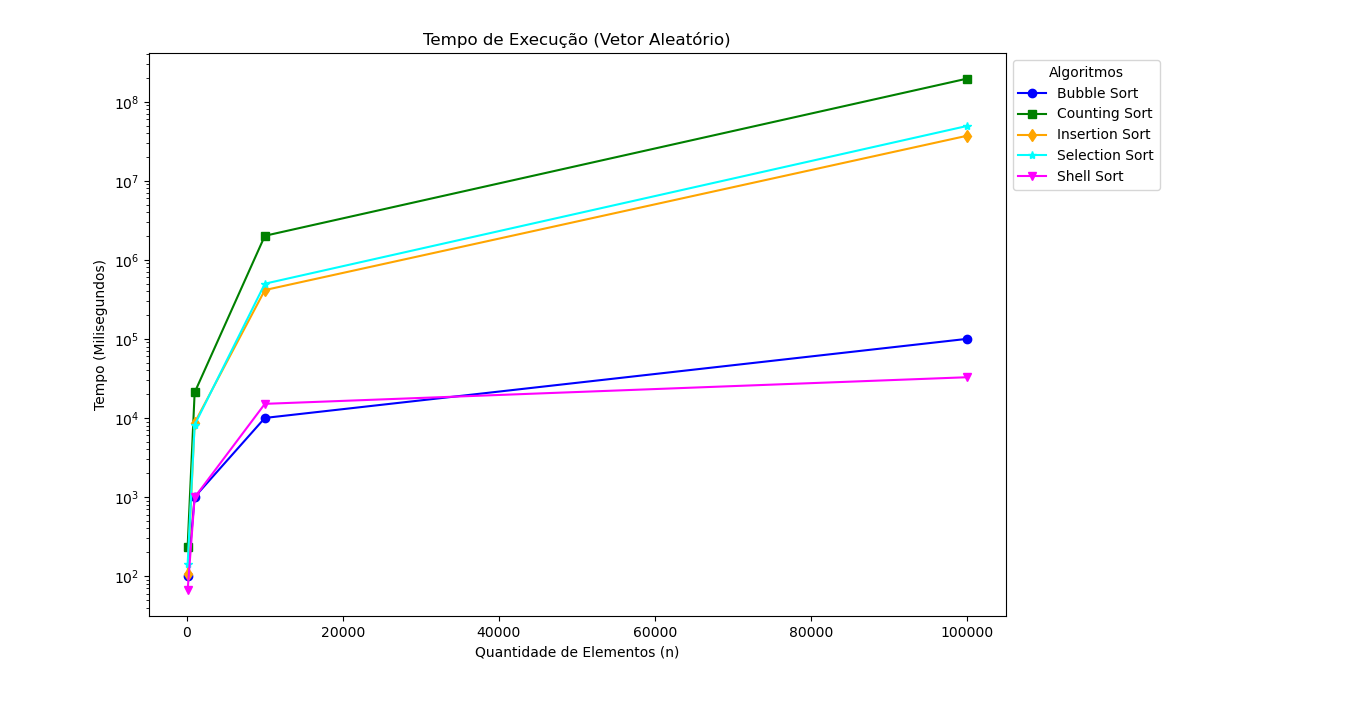
\includegraphics[width=1.1\textwidth]{TempoExecn2.png}
  \caption{Gráfico do tempo de execução dos algoritmos $O(n^2)$}
  \label{fig:1}
\end{figure}

\begin{table}[H]
  \parbox{.45\linewidth}{
    \centering
    \caption{Tabela de tempo BubbleSort}
    \begin{tabular}{|c|c|c|c|c|}
    \hline
    N & Ordenado & Inverso & Aleatório \\ \hline
    100 & 0,0000010 & 0,0000270 & 0,0000284 \\ \hline
    1000 & 0,0000020 & 0,0025190 & 0,0017618 \\ \hline
    10000 & 0,0000100 & 0,1631880 & 0,1288670 \\ \hline
    100000 & 0,0001100 & 16,3827490 & 24,4596327 \\ \hline
    \end{tabular}
  }
  \hfill
  \parbox{.45\linewidth}{
    \centering
    \caption{Tabela de tempo Contagem de Menores}
    \begin{tabular}{|c|c|c|c|c|}
    \hline
    N & Ordenado & Inverso & Aleatório \\ \hline
    100 & 0,0000150 & 0,0000180 & 0,0000236 \\ \hline
    1000 & 0,0011550 & 0,0014480 & 0,0021007 \\ \hline
    10000 & 0,0709920 & 0,0722970 & 0,2012917 \\ \hline
    100000 & 6,7837270 & 6,9611560 & 19,5759227 \\ \hline
    \end{tabular}
  }
\end{table}

\begin{table}[H]
  \parbox{.45\linewidth}{
    \centering
    \caption{Tabela de tempo InsertionSort}
    \begin{tabular}{|c|c|c|c|c|}
    \hline
    N & Ordenado & Inverso & Aleatório \\ \hline
    100 & 0,0000010 & 0,0000190 & 0,0000106 \\ \hline
    1000 & 0,0000040 & 0,0017370 & 0,0008696 \\ \hline
    10000 & 0,0000320 & 0,0781930 & 0,0414341 \\ \hline
    100000 & 0,0001980 & 7,5822750 & 3,7076095 \\ \hline
    \end{tabular}
  }
  \hfill
  \parbox{.45\linewidth}{
    \centering
    \caption{Tabela de tempo SelectionSort}
    \begin{tabular}{|c|c|c|c|c|}
    \hline
    N & Ordenado & Inverso & Aleatório \\ \hline
    100 & 0,0000110 & 0,0000120 & 0,0000140 \\ \hline
    1000 & 0,0008560 & 0,0008950 & 0,0008179 \\ \hline
    10000 & 0,0433020 & 0,0474450 & 0,0498981 \\ \hline
    100000 & 4,5914320 & 4,9460330 & 4,9296037 \\ \hline
    \end{tabular}
  }
\end{table}

\begin{table}[H]
  \centering
  \caption{Tabela de tempo ShellSort}
  \begin{tabular}{|c|c|c|c|c|}
  \hline
  N & Ordenado & Inverso & Aleatório \\ \hline
  100 & 0,0000020 & 0,0000040 & 0,0000066 \\ \hline
  1000 & 0,0000160 & 0,0000360 & 0,0000989 \\ \hline
  10000 & 0,0000970 & 0,0008470 & 0,0015074 \\ \hline
  100000 & 0,0010010 & 0,0381660 & 0,0327194 \\ \hline
  \end{tabular}
\end{table}

\vspace{0.5cm}

\textbf{2.2 $O(n \log(n))$}

\begin{figure}[H]
  \centering
  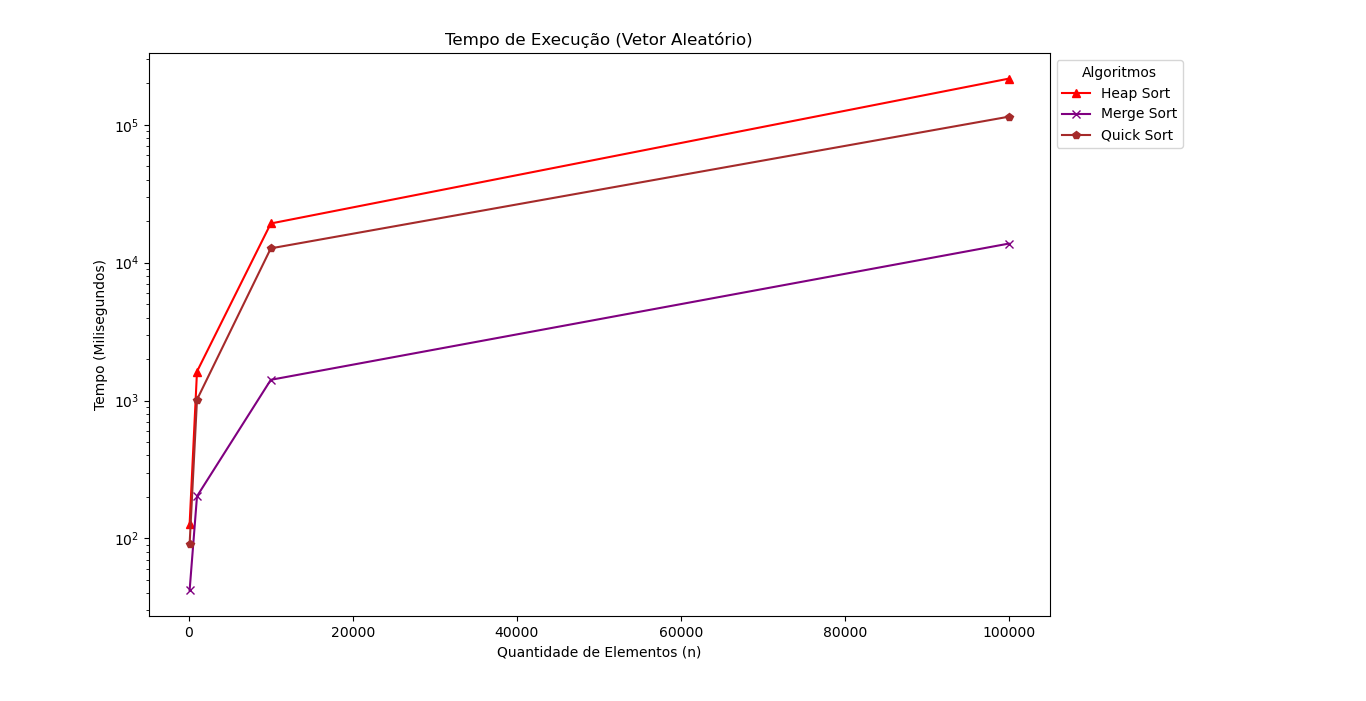
\includegraphics[width=1.1\textwidth]{TempoExecnlogn.png}
  \caption{Gráfico do tempo de execução dos algoritmos $O(n \log(n))$}
  \label{fig:2}
\end{figure}

\begin{table}[H]
  \parbox{.45\linewidth}{
    \centering
    \caption{Tabela de tempo HeapSort}
    \begin{tabular}{|c|c|c|c|c|}
    \hline
    N & Ordenado & Inverso & Aleatório \\ \hline
    100 & 0,0000120 & 0,0000110 & 0,0000127 \\ \hline
    1000 & 0,0001190 & 0,0001320 & 0,0001623 \\ \hline
    10000 & 0,0017670 & 0,0016640 & 0,0019236 \\ \hline
    100000 & 0,0167980 & 0,0160630 & 0,0216151 \\ \hline
    \end{tabular}
  }
  \hfill
  \parbox{.45\linewidth}{
    \centering
    \caption{Tabela de tempo MergeSort}
    \begin{tabular}{|c|c|c|c|c|}
    \hline
    N & Ordenado & Inverso & Aleatório \\ \hline
    100 & 0,0000030 & 0,0000030 & 0,0000042 \\ \hline
    1000 & 0,0000060 & 0,0000100 & 0,0000202 \\ \hline
    10000 & 0,0000420 & 0,0000420 & 0,0001413 \\ \hline
    100000 & 0,0003980 & 0,0003860 & 0,0013745 \\ \hline
    \end{tabular}
  }
\end{table}

\begin{table}[H]
  \centering
  \caption{Tabela de tempo QuickSort}
  \begin{tabular}{|c|c|c|c|c|}
  \hline
  N & Ordenado & Inverso & Aleatório \\ \hline
  100 & 0,0000060 & 0,0000090 & 0,0000091 \\ \hline
  1000 & 0,0000310 & 0,0003190 & 0,0001015 \\ \hline
  10000 & 0,0005380 & 0,0287280 & 0,0012698 \\ \hline
  100000 & 0,0040020 & 2,6863460 & 0,0114474 \\ \hline
  \end{tabular}
\end{table}

\vspace{0.5cm}

\textbf{2.3 $O(n k)$}

\begin{figure}[H]
  \centering
  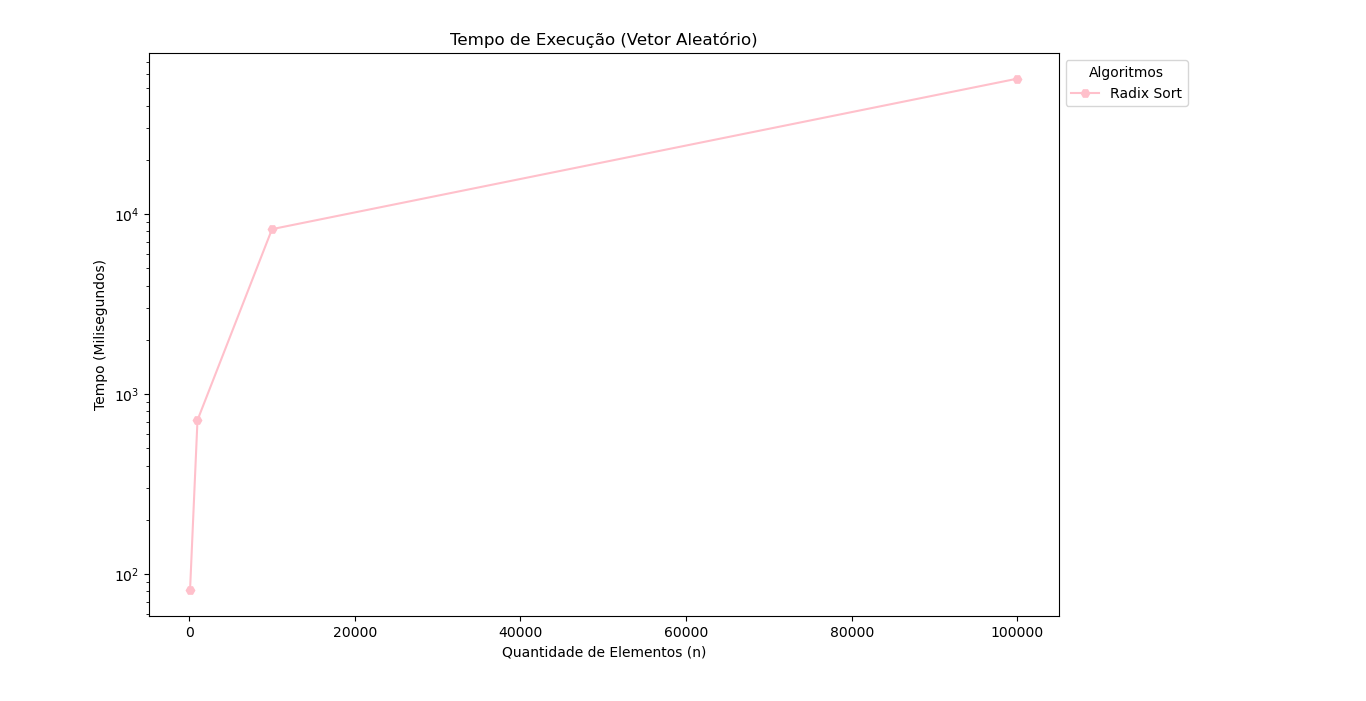
\includegraphics[width=1.1\textwidth]{TempoExecnk.png}
  \caption{Gráfico do tempo de execução dos algoritmos $O(n k)$}
  \label{fig:3}
\end{figure}

\begin{table}[H]
  \centering
  \caption{Tabela de tempo RadixSort}
  \begin{tabular}{|c|c|c|c|c|}
  \hline
  N & Ordenado & Inverso & Aleatório \\ \hline
  100 & 0,0000080 & 0,0000080 & 0,0000081 \\ \hline
  1000 & 0,0000760 & 0,0000750 & 0,0000715 \\ \hline
  10000 & 0,0004810 & 0,0009150 & 0,0008243 \\ \hline
  100000 & 0,0056120 & 0,0061550 & 0,0056570 \\ \hline
  \end{tabular}
\end{table}

\vspace{0.25cm}

\textbf{3. Quantidade de Comparações}

\vspace{0.5cm}

\textbf{3.1 $O(n^2)$}

\begin{table}[H]
  \parbox{.45\linewidth}{
    \centering
    \caption{Tabela de comparações BubbleSort}
    \begin{tabular}{|c|c|c|c|c|}
    \hline
    N & Ordenado & Inverso & Aleatório \\ \hline
    100 & 99 & 4950 & 4882,1 \\ \hline
    1000 & 999 & 499500 & 498700,7 \\ \hline
    10000 & 9999 & 49995000 & 49987304,1 \\ \hline
    100000 & 99999 & 4999950000 & 4999798132 \\ \hline
    \end{tabular}
  }
  \hfill
  \parbox{.45\linewidth}{
    \centering
    \caption{Tabela de comparações Contagem de Menores}
    \begin{tabular}{|c|c|c|c|c|}
    \hline
    N & Ordenado & Inverso & Aleatório \\ \hline
    100 & 4950 & 4950 & 4950 \\ \hline
    1000 & 499500 & 499500 & 499500 \\ \hline
    10000 & 49995000 & 49995000 & 49995000 \\ \hline
    100000 & 4999950000 & 4999950000 & 4999950000 \\ \hline
    \end{tabular}
  }
\end{table}

\begin{table}[H]
  \parbox{.45\linewidth}{
    \centering
    \caption{Tabela de comparações InsertionSort}
    \begin{tabular}{|c|c|c|c|c|}
    \hline
    N & Ordenado & Inverso & Aleatório \\ \hline
    100 & 99 & 4950 & 2636,3 \\ \hline
    1000 & 999 & 499500 & 249352,9 \\ \hline
    10000 & 9999 & 49995000 & 24986288,7 \\ \hline
    100000 & 99999 & 4999950000 & 2498975066 \\ \hline
    \end{tabular}
  }
  \hfill
  \parbox{.45\linewidth}{
    \centering
    \caption{Tabela de comparações SelectionSort}
    \begin{tabular}{|c|c|c|c|c|}
    \hline
    N & Ordenado & Inverso & Aleatório \\ \hline
    100 & 4950 & 4950 & 4950 \\ \hline
    1000 & 499500 & 499500 & 499500 \\ \hline
    10000 & 49995000 & 49995000 & 49995000 \\ \hline
    100000 & 4999950000 & 4999950000 & 4999950000 \\ \hline
    \end{tabular}
  }
\end{table}

\begin{table}[H]
  \centering
  \caption{Tabela de comparações ShellSort}
  \begin{tabular}{|c|c|c|c|c|}
  \hline
  N & Ordenado & Inverso & Aleatório \\ \hline
  100 & 0 & 414 & 573,7 \\ \hline
  1000 & 0 & 5188 & 11295,2 \\ \hline
  10000 & 0 & 211340 & 252463,5 \\ \hline
  100000 & 0 & 18184250 & 11965729,8 \\ \hline
  \end{tabular}
\end{table}

\vspace{0.5cm}

\textbf{3.2 $O(n \log(n))$}

\begin{table}[H]
  \parbox{.45\linewidth}{
    \centering
    \caption{Tabela de comparações HeapSort}
    \begin{tabular}{|c|c|c|c|c|}
    \hline
    N & Ordenado & Inverso & Aleatório \\ \hline
    100 & 1380 & 1132 & 1262,2 \\ \hline
    1000 & 20416 & 17632 & 19143,2 \\ \hline
    10000 & 273912 & 243392 & 258448,2 \\ \hline
    100000 & 3401708 & 3094868 & 3249879,6 \\ \hline
    \end{tabular}
  }
  \hfill
  \parbox{.45\linewidth}{
    \centering
    \caption{Tabela de comparações MergeSort}
    \begin{tabular}{|c|c|c|c|c|}
    \hline
    N & Ordenado & Inverso & Aleatório \\ \hline
    100 & 99 & 102 & 188,9 \\ \hline
    1000 & 999 & 1001 & 1981,3 \\ \hline
    10000 & 9999 & 10005 & 19977,4 \\ \hline
    100000 & 99999 & 100006 & 199975,4 \\ \hline
    \end{tabular}
  }
\end{table}

\begin{table}[H]
  \centering
  \caption{Tabela de comparações QuickSort}
  \begin{tabular}{|c|c|c|c|c|}
  \hline
  N & Ordenado & Inverso & Aleatório \\ \hline
  100 & 756 & 1417 & 873,9 \\ \hline
  1000 & 10814 & 102188 & 12786,1 \\ \hline
  10000 & 141660 & 9744569 & 178437,5 \\ \hline
  100000 & 1747098 & 968505521 & 2232338,6 \\ \hline
  \end{tabular}
\end{table}

\vspace{0.5cm}

\textbf{3.3 $O(n k)$}

\begin{table}[H]
  \centering
  \caption{Tabela de comparações RadixSort}
  \begin{tabular}{|c|c|c|c|c|}
  \hline
  N & Ordenado & Inverso & Aleatório \\ \hline
  100 & 100 & 100 & 100 \\ \hline
  1000 & 1000 & 1000 & 1000 \\ \hline
  10000 & 10000 & 10000 & 10000 \\ \hline
  100000 & 100000 & 100000 & 100000 \\ \hline
  \end{tabular}
\end{table}

\vspace{0.25cm}

\textbf{4. Movimentações}

\vspace{0.5cm}

\textbf{4.1 $O(n^2)$}

\begin{table}[H]
  \parbox{.45\linewidth}{
    \centering
    \caption{Tabela de trocas BubbleSort}
    \begin{tabular}{|c|c|c|c|c|}
    \hline
    N & Ordenado & Inverso & Aleatório \\ \hline
    100 & 0 & 4950 & 2542,9 \\ \hline
    1000 & 0 & 499500 & 248360,4 \\ \hline
    10000 & 0 & 49995000 & 24976298,5 \\ \hline
    100000 & 0 & 4999950000 & 2271704616 \\ \hline
    \end{tabular}
  }
  \hfill
  \parbox{.45\linewidth}{
    \centering
    \caption{Tabela de trocas Contagem de Menores}
    \begin{tabular}{|c|c|c|c|c|}
    \hline
    N & Ordenado & Inverso & Aleatório \\ \hline
    100 & 100 & 100 & 100 \\ \hline
    1000 & 1000 & 1000 & 1000 \\ \hline
    10000 & 10000 & 10000 & 10000 \\ \hline
    100000 & 100000 & 100000 & 100000 \\ \hline
    \end{tabular}
  }
\end{table}

\begin{table}[H]
  \parbox{.45\linewidth}{
    \centering
    \caption{Tabela de trocas InsertionSort}
    \begin{tabular}{|c|c|c|c|c|}
    \hline
    N & Ordenado & Inverso & Aleatório \\ \hline
    100 & 99 & 5049 & 2641,9 \\ \hline
    1000 & 999 & 500499 & 249359,4 \\ \hline
    10000 & 9999 & 50004999 & 24986297,5 \\ \hline
    100000 & 99999 & 5000049999 & 2498975077 \\ \hline
    \end{tabular}
  }
  \hfill
  \parbox{.45\linewidth}{
    \centering
    \caption{Tabela de trocas SelectionSort}
    \begin{tabular}{|c|c|c|c|c|}
    \hline
    N & Ordenado & Inverso & Aleatório \\ \hline
    100 & 0 & 50 & 94,7 \\ \hline
    1000 & 0 & 500 & 993,6 \\ \hline
    10000 & 0 & 5000 & 9991,5 \\ \hline
    100000 & 0 & 50000 & 99987,8 \\ \hline
    \end{tabular}
  }
\end{table}

\begin{table}[H]
  \centering
  \caption{Tabela de trocas ShellSort}
  \begin{tabular}{|c|c|c|c|c|}
  \hline
  N & Ordenado & Inverso & Aleatório \\ \hline
  100 & 291 & 705 & 864,7 \\ \hline
  1000 & 4610 & 9798 & 15905,2 \\ \hline
  10000 & 49610 & 260950 & 302073,5 \\ \hline
  100000 & 499610 & 18683860 & 12465339,8 \\ \hline
  \end{tabular}
\end{table}

\vspace{0.5cm}

\textbf{4.2 $O(n \log(n))$}

\begin{table}[H]
  \parbox{.45\linewidth}{
    \centering
    \caption{Tabela de trocas HeapSort}
    \begin{tabular}{|c|c|c|c|c|}
    \hline
    N & Ordenado & Inverso & Aleatório \\ \hline
    100 & 640 & 516 & 581,1 \\ \hline
    1000 & 9708 & 8316 & 9071,6 \\ \hline
    10000 & 131956 & 116696 & 124224,1 \\ \hline
    100000 & 1650854 & 1497434 & 1574939,8 \\ \hline
    \end{tabular}
  }
  \hfill
  \parbox{.45\linewidth}{
    \centering
    \caption{Tabela de trocas MergeSort}
    \begin{tabular}{|c|c|c|c|c|}
    \hline
    N & Ordenado & Inverso & Aleatório \\ \hline
    100 & 201 & 201 & 201 \\ \hline
    1000 & 2000 & 2000 & 2000 \\ \hline
    10000 & 20004 & 20004 & 20004 \\ \hline
    100000 & 200005 & 200005 & 200005 \\ \hline
    \end{tabular}
  }
\end{table}

\begin{table}[H]
  \centering
  \caption{Tabela de trocas QuickSort}
  \begin{tabular}{|c|c|c|c|c|}
  \hline
  N & Ordenado & Inverso & Aleatório \\ \hline
  100 & 424 & 1179 & 482 \\ \hline
  1000 & 5840 & 99206 & 6731,8 \\ \hline
  10000 & 75580 & 9709257 & 93351,2 \\ \hline
  100000 & 919107 & 968096337 & 1164047,7 \\ \hline
  \end{tabular}
\end{table}

\vspace{0.5cm}

\textbf{4.3 $O(n k)$}

\begin{table}[H]
  \centering
  \caption{Tabela de trocas RadixSort}
  \begin{tabular}{|c|c|c|c|c|}
  \hline
  N & Ordenado & Inverso & Aleatório \\ \hline
  100 & 300 & 300 & 300 \\ \hline
  1000 & 4000 & 4000 & 4000 \\ \hline
  10000 & 50000 & 50000 & 50000 \\ \hline
  100000 & 600000 & 600000 & 600000 \\ \hline
  \end{tabular}
\end{table}

\vspace{0.25cm}

\textbf{5. Análise dos Resultados}

Na necessidade de dicidir qual o melhor e o pior algoritmo, vamos nos aproximar o máximo possível de uma situação real, onde a propriedade que mais importa é o \textbf{tempo de execução}, que pode ser o gargalo para outros serviços, e não a quantidade de trocas ou comparações, tendo em vista a alta capacidade computacional das máquinas atuais. Além disso, o vetor que mais se aproxima de situações reais é um \textbf{aleatório}. Portanto, vamos analisar o gráfico a seguir.

\begin{figure}[H]
  \centering
  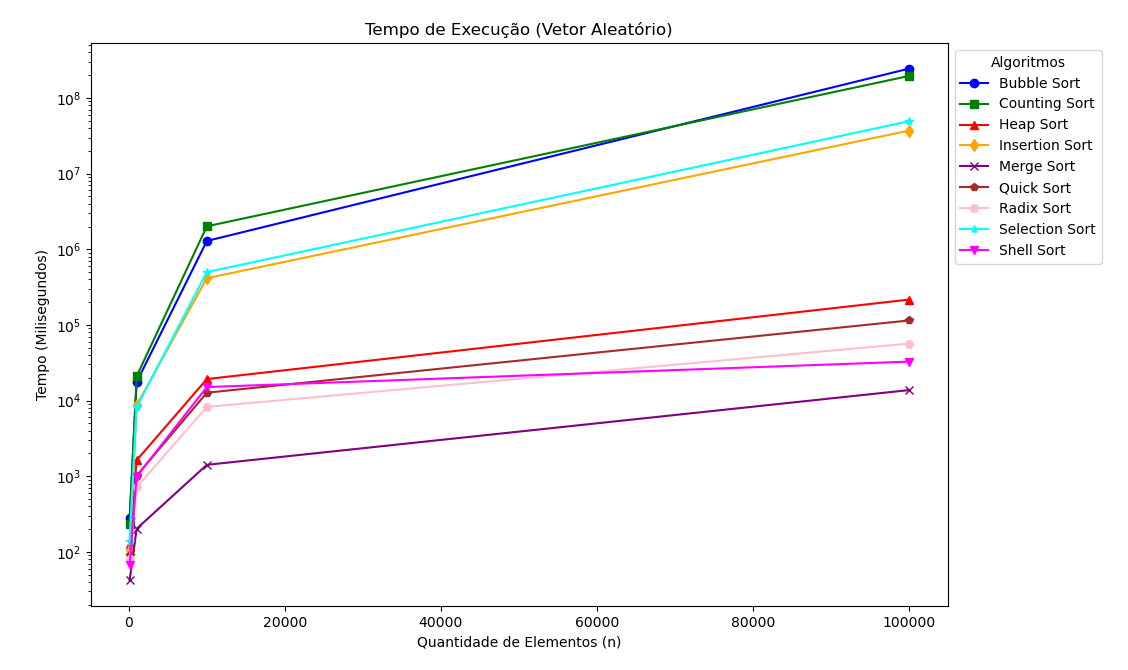
\includegraphics[width=1\textwidth]{TempoExecGeralAleat2.png}
  \caption{Gráfico do tempo de execução de todos algoritmos}
  \label{fig:4}
\end{figure}

Percebemos, no gráfico, que o melhor algoritmo foi o \textbf{MergeSort}, enquanto os piores foram o \textbf{BubbleSort} e o \textbf{Contagem de Menores}. Esse resultado faz sentido quando comparado com as complexidades dos algoritmos, visto que o MergeSort tem complexidade temporal $O(n \log(n))$. Note, contudo, que ele possui uma complexidade de espaço $O(n)$. Os piores algoritmos foram aqueles com complexidade temporal $O(n^2)$, com complexidades espaciais de $O(n)$.

\vspace{0.25cm}

\end{document}